% titlepage-demo.tex
\documentclass{beamer}
\usetheme{Boadilla}
\usepackage{multirow}
\usepackage[absolute,overlay]{textpos} 
\newenvironment{reference}[2]{% 
  \begin{textblock*}{\textwidth}(#1,#2) 
      \footnotesize\it\bgroup\color{red!50!black}}{\egroup\end{textblock*}} 



\begin{document}

\begin{frame}{Appendix 1 - Future Work} 	
	
\begin{itemize}
	\item Learning the relationship between segments.
	\begin{itemize}
		\item We have not imposed any constraints on the relationship between segments.
		\item However, spatial-temporal relationship might
		be important to identify an event. 
		\item For example, in the event ``changing a vehicle tire'',
		the action ``removing hubcap'' should take place before the action ``replacing tire''.
	\end{itemize}
	\item Learning the importance of each concept in the concept bank.
	\begin{itemize}
		\item Concepts are obtained from the event description.
		\item We do not know if it really visually represents for that event.
		\\
		$\rightarrow$ which	concepts that both textually and visually represent for an event?	
	\end{itemize}
	\item Video description generation.
	\begin{itemize}
		\item Generate textual descriptions for video.
		\item Many potential applications such as helping blind people understand what is happening in a video.
	\end{itemize}
\end{itemize}
	
\end{frame}	

\begin{frame}{Appendix 2 - Segment-based Representation} 	
	
	\begin{center}
		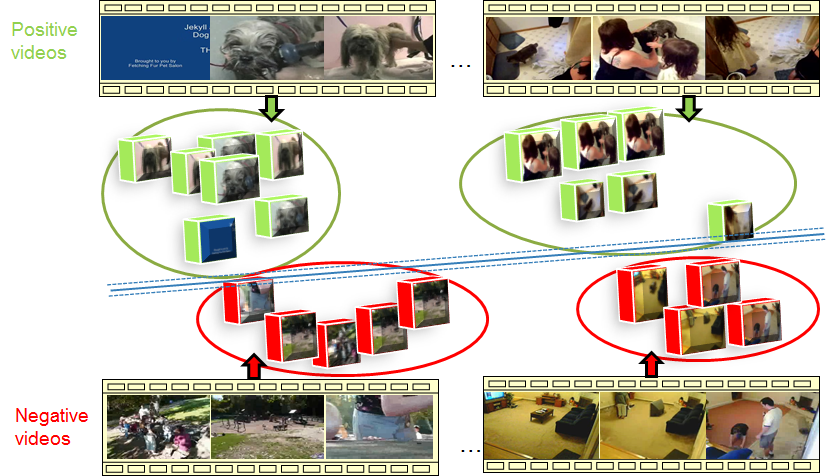
\includegraphics[width=11cm,height=6cm]{images/part4/segmentbased.png}
	\end{center}
	
\end{frame}	

\begin{frame}{Appendix 3 - Results of Segment-based on MED 2011 (linear SVM, sum aggregation)} 	
	
	\begin{center}
		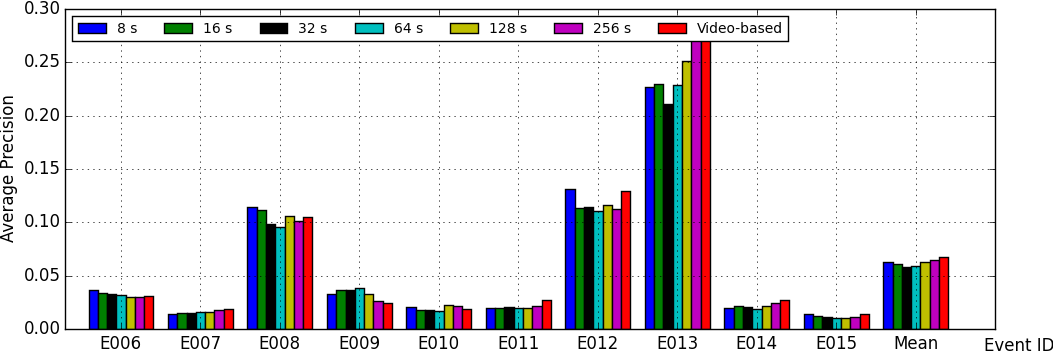
\includegraphics[width=11cm,height=5cm]{images/part4/sb_linear_sum.png}
	\end{center}
	
\end{frame}	

\begin{frame}{Appendix 4 - Results of Segment-based on MED 2011 (linear SVM, max aggregation)} 	
	
	\begin{center}
		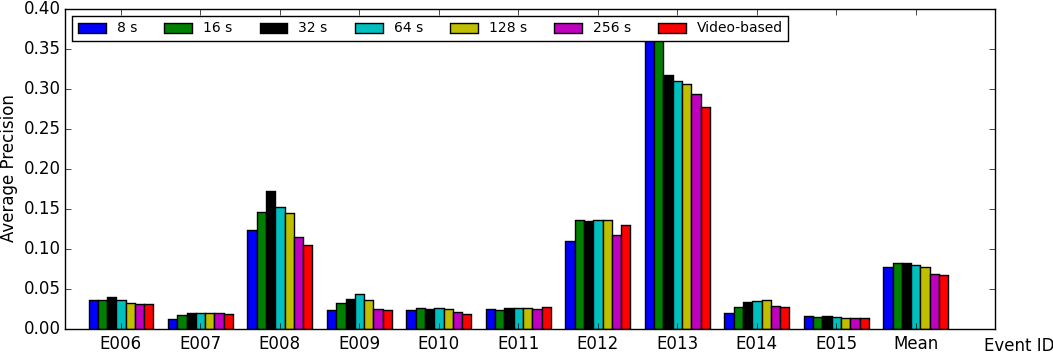
\includegraphics[width=11cm,height=5cm]{images/part4/sb_linear_max.png}
	\end{center}
	
\end{frame}	

\begin{frame}{Appendix 5 - Results of Sum-Max video pooling on MED 2011 (linear SVM)} 	
	
	\begin{center}
		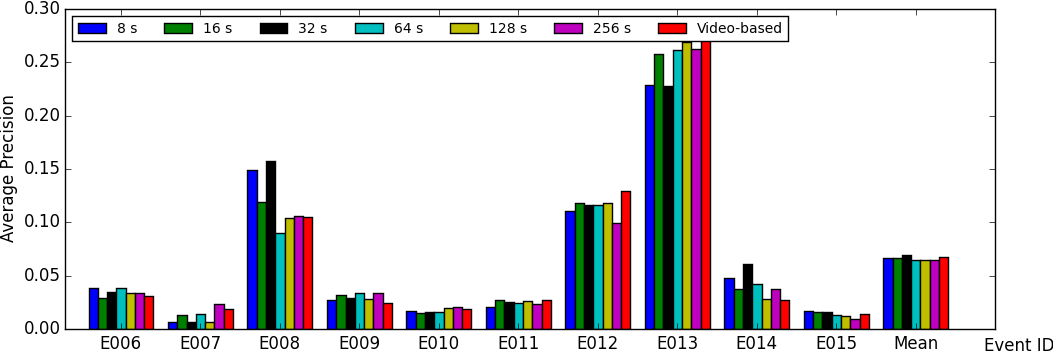
\includegraphics[width=11cm,height=5cm]{images/part4/summax_linear.png}
	\end{center}
	
\end{frame}	


\begin{frame}{Appendix 6 - Comparation with other reported results} 	
	\begin{itemize}
		\item Dataset: MED11
		\item Linear SVM
		\item In terms of mAP (\%)
	\end{itemize}
\begin{table}[h]
	\tiny
	\begin{tabular}{@{}|c|c|c|c|c|l|c|c|@{}}
		\toprule
		\begin{tabular}[c]{@{}c@{}}Tang\\ CVPR2011\end{tabular} & \begin{tabular}[c]{@{}c@{}}Cao\\ ECCV2012\\ (Linear-SAP)\end{tabular} & \begin{tabular}[c]{@{}c@{}}Vahdat\\ ICCV2013\\ (Linear-LSVM)\end{tabular} & \begin{tabular}[c]{@{}c@{}}Vahdat\\ ICCV2013\\ (Kernel-LSVM)\end{tabular} & \begin{tabular}[c]{@{}c@{}}Lai\\ CVPR2014\\ s-pSVM\end{tabular} & \begin{tabular}[c]{@{}l@{}}Lai\\ CVPR2014\\ m-pSVM\end{tabular} & \begin{tabular}[c]{@{}c@{}}Mori\\ CVPR2015\end{tabular} & \begin{tabular}[c]{@{}c@{}}Ours\\ (EDMIL)\end{tabular} \\ \midrule
		4.77                                                    & 6.28                                                                  & 3.19                                                                      & \textit{11.22}                                                                     & 4.3                                                             & 5.0                                                             & 6.1                                                     & \textbf{9.68}                                                   \\ \bottomrule
	\end{tabular}
\end{table}
	
\end{frame}	


\end{document}